\section{Part 1: Core Features}
This section details the core features implemented in the project. This includes converting the dataset to a suitable file format and summarizing a few key statistics about the dataset.

\subsection{Feature Description}
The following section details each of the core features implemented in the project.

\paragraph{Task 1: Read in and store the dataset using PySpark.} This task involves reading in the dataset and storing it using PySpark.The dataset is read in from \textit{airline.csv}, which has a file size of over \textgreater 80GB, using PySpark. The dataset is then stored in in the Parquet file format \cite{parquet}. Parquet is a columnar storage format the provides efficient storage and encoding of data. Parquet utilizes the algorithm outlined in Dremel, an interactive query system for analysis of read-only nested data \cite{36632}, to represent nested structures. This algorithm can be broken down into two individual algorithms: the column stripping algorithm, which transforms complex records into a columnar format, and the record assembly algorithm, which reconstructs the original records from these columns when needed. Column stripping allows for better compression than traditional row-oriented storage formats, such as CSV, by exploiting the redundancy in the data found within columns of data, skipping non-relevant data very quickly \cite{Databricks}. Meanwhile, he row assembly algorithm ensures that despite the high compression, the data can be reconstructed quickly when needed, which is essential for large datasets such as the one used in the project, where I/O operations can be a bottleneck. By storing the dataset in Parquet format, the amount of data read from disk is minimized, and the data is stored in a more efficient manner, allowing for faster query times and better performance overall. The benefits of the Parquet format as opposed to CSV are outlined in Figure \ref{fig:parquet_vs_csv} below.

\begin{figure}[H]
  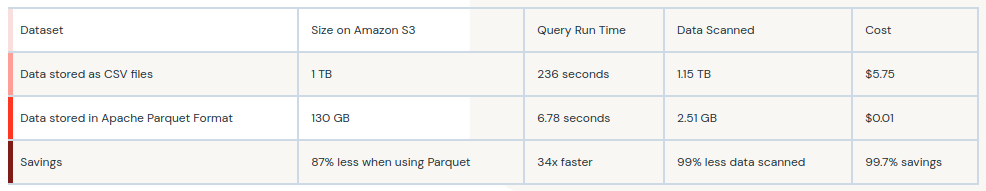
\includegraphics[width=\linewidth]{parquet_vs_csv.png}
  \caption{Comparison of Parquet and CSV file formats in terms of file size, query run time, data scanned and cost \cite{Databricks}.}
  \label{fig:parquet_vs_csv}
\end{figure}

\noindent \textit{Location:} Code lines 13-27 in file \codeword{backend/scripts/convert.py}

\paragraph{Task 2: Display the total number of flights for a given year.} This task allows the user to specify a year and view the total number of flights that occurred in that year. This is done by filtering the airline dataframe based on the specified year and counting the number of rows in the resulting dataframe.\\

\noindent \textit{Location:} Code lines 26-36 in file \codeword{backend/part1/views.py}

\paragraph{Task 3: Display the total number of flights given a range of years.} This task allows the user to specify a start year and end year and view the total number of flights that occurred within that range. This is done by filtering the airline dataframe based on the specified range of years and counting the number of rows in the resulting dataframe.\\

\noindent \textit{Location:} Code lines 52-69 in file \codeword{backend/part1/views.py}

\paragraph{Task 4: Display the total number of flights given a list of years.} This task allows the user to specify a list of years and view the total number of flights that occurred in each year. This is done by filtering the airline dataframe based on the specified list of years using the \codeword{isin()} function and counting the number of rows in the resulting dataframe for each year.\\

\noindent \textit{Location:} Code lines 83-97 in file \codeword{backend/part1/views.py}

\paragraph{Task 4: Display the timeliness percentage of flights for a given year.} This task allows the user to specify a year and view the percentage of flights that departed on time, early, and late. The 'DepDelay' column is used to determine the timeliness of flights, with flights that departed on time having a 'DepDelay' of 0, flights that departed early having a 'DepDelay' less than 0, and flights that departed late having a 'DepDelay' greater than 0. Flight with an unknown departure delay are determined by subtracting the number of flights that departed on time, early, and late from the total number of flights. The percentage of flights in each category is then calculated and displayed to the user in the form of a pie chart.\\

\noindent \textit{Location:} Code lines 115-149 in file \codeword{backend/part1/views.py}

\paragraph{Task 5: Display the top reason for cancelled flights for a given year.} This task allows the user to specify a year and view the top reason for cancelled flights in that year. This is done by filtering the airline dataframe based on the specified year and creating a new dataframe that groups the data by the 'CancellationCode' column and counts the number of occurrences of each cancellation code. The cancellation code with the highest count is then displayed to the user.\\

\noindent \textit{Location:} Code lines 163-193 in file \codeword{backend/part1/views.py}

\paragraph{Task 6: Display the top 3 most punctual airports for a given year} This task allows the user to specify a year and view the top 3 airports with the most punctual flights in that year. This is done by filtering the airline dataframe based on the specified year and creating a new dataframe aggregates this to data to calculate the median departure delay (using the 'DepDelay' column) for each airport. The median is used here as it is less affected by extreme values than the mean, making it more robust to outliers. The top 3 airports with the lowest median departure delay are then displayed to the user.\\

\noindent \textit{Location:} Code lines 207-238 in file \codeword{backend/part1/views.py}

\paragraph{Task 7: Display the top 3 worst performing airlines} This task allows the user to view the top 3 worst performing airlines of the twentieth century based on a performance metric. The performance metric takes into account three factors:

\begin{itemize}
    \item The percentage of flights that were delayed when departing.
    \item The percentage of flights that were delayed when arriving.
    \item The percentage of flights that were cancelled.
\end{itemize}

\noindent The dataframe is first filtered to include only flights that occurred in the twentieth century. The performance metric is then calculated for each airline by aggregating the data based on the\\ 'DOT\_ID\_Reporting\_Airline' column. Finally, a composite percentage score is calculated for each airline based on the three factors mentioned above by taking the average of the three percentages. The top 3 airlines with the highest composite percentage score are then displayed to the user.\\

\noindent \textit{Location:} Code lines 247-268 in file \codeword{backend/part1/views.py}
